\documentclass[12pt,a4paper]{article}
\usepackage[utf8]{inputenc}
\usepackage[russian]{babel}
\usepackage[OT1]{fontenc}
\usepackage{graphicx}
\usepackage{calc}
\usepackage[margin=15mm]{geometry}
\usepackage{cmap}

% условие без картинки
\newcommand{\task}[2]{
\hrule
\hbox to \textwidth {%
     \vrule
\parbox[t]{0.04\textwidth}{\smallskip \centering #1}%
     \vrule%
\hfill%
     \parbox[t]{0.93\textwidth}{\smallskip #2 \smallskip}\hfill%
\vrule
}
\hrule
    \pagebreak[2]
}

\newlength{\h}
\newsavebox{\taskbox}
\newlength{\x}
\newsavebox{\pictbox}

% условие с картинкой (картинка выравнивается по центру)
\newcommand{\taskpic}[3]{
\savebox{\taskbox}{\parbox[t]{0.93\textwidth-4.3cm}{\smallskip #2 \smallskip}}
\savebox{\pictbox}{\parbox[t]{4cm}{\smallskip \centering
     \vspace{0pt} #3 \smallskip}}
\h=\ht\taskbox
\advance\h\dp\taskbox
\x=\ht\pictbox
\advance\x\dp\pictbox
\hrule
\hbox to \textwidth {%
\vrule\parbox[t][\maxof{\h}{\x}][t]{0.04\textwidth}{ \smallskip
     \centering #1 }\vrule%
\hfill\parbox[t][\maxof{\h}{\x}][t]{0.93\textwidth-4.3cm}{\smallskip #2
     \smallskip}\hfill\vrule%
\hfill\parbox[t][\maxof{\h}{\x}][c]{4cm}{\hfil #3 \hfil}\hfill\vrule
}
\hrule
\pagebreak[2]
}
\pagestyle{empty}
\graphicspath{ {images/} }

\begin{document}

\begin{center}
\begin{Large}
\textsc{ГЦФО. 9 класс. 2014/15.}
\end{Large}
\end{center}

\small

\taskpic{39}{Легкий жгут жесткости $k$ прикреплен к потолку, а на его конце висят два жука (см. рис.). В таком положении жгут равномерно растянут и его длина от потолка до жуков равна $l$. Потом один жук начинает карабкаться по жгуту вверх с постоянной сокростью $v$ относительно жгута. Как и с какой скоростью относительно потолка будет двигаться второй жук, который продолжает держаться за конец жгута. Считать, что каждый жук хватается за жгут в одной точке. Масса обоих жуков равна $m$, их размерами пренебречь. Ускорение свободного падения равно $g$.}{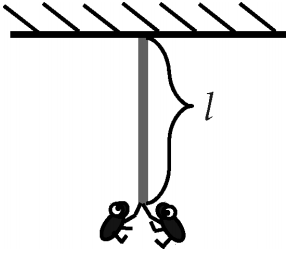
\includegraphics[width=4cm]{39}}
\taskpic{40}{Два одинаковых проводящих проволочных кольца радиуса $a$ сварили в противоположных точках O и O' как указано на рисунке. Сопротивление единицы длины проволоки равно $\lambda$. Дуги AO и BO равны, их длина $l$. Найти зависимость сопротивления между точками A и B от величины $l$.}{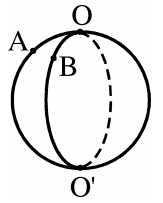
\includegraphics[width=2cm]{40}}
\task{41}{Поршень массы $M = 2$~кг может с трением скользить внутри вертикальной неподвижной трубы. Сначала поршень прикрепили внутри трубы к потолку пружиной жесткостью $k_1 = 20$~Н/м, длина которой в нерастянутом состоянии $l_1=60$~см. Поршень расположили на уровне середины трубы, отпустили, и он остался неподвижен. Затем опыт повторили, поменяв пружину - жесткость новой пружины стала $k_2 = 10$~Н/м, а длина в нерастянутом состоянии $l_2 = 20$~см. Удивительно, но поршень в середине трубы снова остался неподвижен. При каких значениях силы трения поршня о трубу это возможно? Влиянием воздуха пренебречь, $g = 10$~м/с$^2$.}
\taskpic{43}{Велосипед с колесами, имеющими форму равностороннего треугольника, за время $t$ прошел по дороге достаточно большое расстояние $s$. Найдите среднее значение модуля скорости точки, расположенной в вершине колеса. Колеса не проскальзывают по дороге, велосипед не отрывается от земли.}{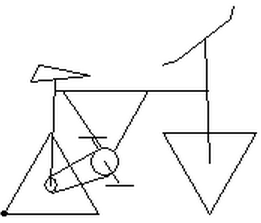
\includegraphics[width=3cm]{43}}
\taskpic{44}{Экспериментатор взял 4 одинаковых металлических стержня и собрал из них Y-образную фигуру. К концам фигуры экспериментатор присоединил 3 одинаковых больших металлических шара, имеющих температуру $t_1 = 0 ^\circ$C, $t_2 = 50 ^\circ$C и $t_3 = 100 ^\circ$C (см. рис.). Экспериментатор обеспечил хороший тепловой контакт стержней с шарами и другими стержнями. Через некоторое время он обнаружил, что первый шар нагрелся на $0{,}4^\circ$C. Какую температуру имели в этот момент два других шара? Считайте, что теплоемкость стержней пренебрежимо мала, а теплообмен с окружающей средой отсутствует. Мощность теплопередачи по стержню пропорциональна разности температур на его концах.}{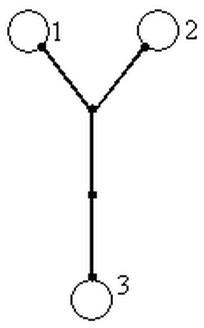
\includegraphics[width=3cm]{44}}
\taskpic{45}{Маленький шарик массы $m$, закрепленный на вертикальной пружине, расположили под столом с отверстием, в положении равновесия шарик находится посередине отверстия. Обнаружилось, что если шарик отклонить вниз на произвольное расстояние и отпустить, он колеблется вокруг положения равновесия с периодом $T_0$. Над отверстием поставили тело массой $m$ (см. рис.) и снова вывели шарик из положения равновесия. Определить период колебаний системы, если известно, что максимальная скорость шарика $v_m$. Шарик и тело соударяются абсолютно упруго; тело, подскакивая, движется строго вертикально. Сопротивлением воздуха пренебречь, ускорение свободного падения~$g$.}{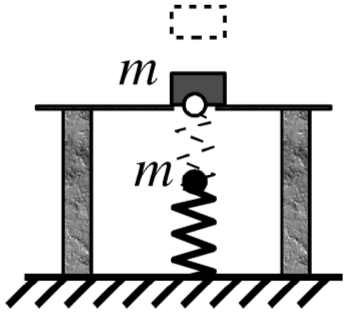
\includegraphics[width=4cm]{45}}

\end{document}
